\chapter{交易金额隐匿技术介绍}

在区块链中,交易金额隐匿是一项可以保护区块链用户隐私的重要技术。
由于区块链的去中心化特性,所有人都有权利查看链上的内容。以比特币为例,
一笔交易的金额被明文写在了交易信息中,这就导致了在隐私方面存在风险,
使其和真正的货币存在区别。真正的货币在交易完成后就难以调查持有货币的上家,
交易的具体金额只有参与交易的少数人知道,每个人所拥有货币的数量也不会公开。
从隐私保护方面来看,在区块链中明文存储交易金额会带来以下隐私风险:
\begin{itemize}
    \item 双方进行交易的金额完全公开,导致任何人都能知道这笔交易的具体数额。
    在很多交易中,交易金额是很重要的机密,例如个人工作月收入、公司间签订合同的金额大小。
    如果交易金额必须公开,就导致类似交易无法使用数字货币进行。
    \item 每个钱包所拥有的货币数量完全公开。由于交易目标都是透明的,
    通过查看和分析所有区块链上的交易就可以轻松计算出每个钱包所拥有的货币数量。
    虽然我们可以通过使用大量不同钱包的方式来缓解这种信息泄露,
    但是这样也带来了使用上的不便,且难以同时使用所有钱包的金额,
    因为这样就会直接暴露这些钱包是由同一个人控制的。
    \item 虚拟货币流向可以完全溯源。为了避免交易被追踪,
    将虚拟货币经过多个钱包转移是一种思路,然而由于区块链上每一笔交易都是透明的,
    我们可以对每一枚数字货币溯源,直至货币刚被开采出来的时候。
    例如有很多网站都在追踪虚拟货币持有大户的动态,一旦大户开始动用持有的货币就会第一时间报导,
    变得人尽皆知。
\end{itemize}

上述隐私风险有部分可以通过隐藏交易双方来解决,但是隐藏交易金额也是很重要的。
由于加密货币可以精确到小数点后八位甚至更多,如果不隐藏交易,
通过具体的交易金额就很容易发现该交易所属的原始交易金额。
虽然可以使用限制链上交易的合法金额的方法让所有交易的金额看起来都很接近,
但是这就需要将一笔交易拆分成非常多笔,而且在交易总量少的情况下依然存在隐私泄露风险。
因此,设计一种可以完全隐匿交易金额的算法是十分重要的。

在隐匿交易金额的同时,为了防止恶意交易,
区块链观察者,尤其是区块链矿工需要能够可靠的验证交易的合法性。为了达成上述目标,
我们需要使用零知识证明方法证明创建交易金额的合法性,
使交易金额得以隐藏的同时,观察者可以验证该交易不包含金额双花、交易输入输出不等、
消费了无权动用的资金、资金金额上溢等问题。

\section{数字货币的交易}

\begin{figure}
    \centering
    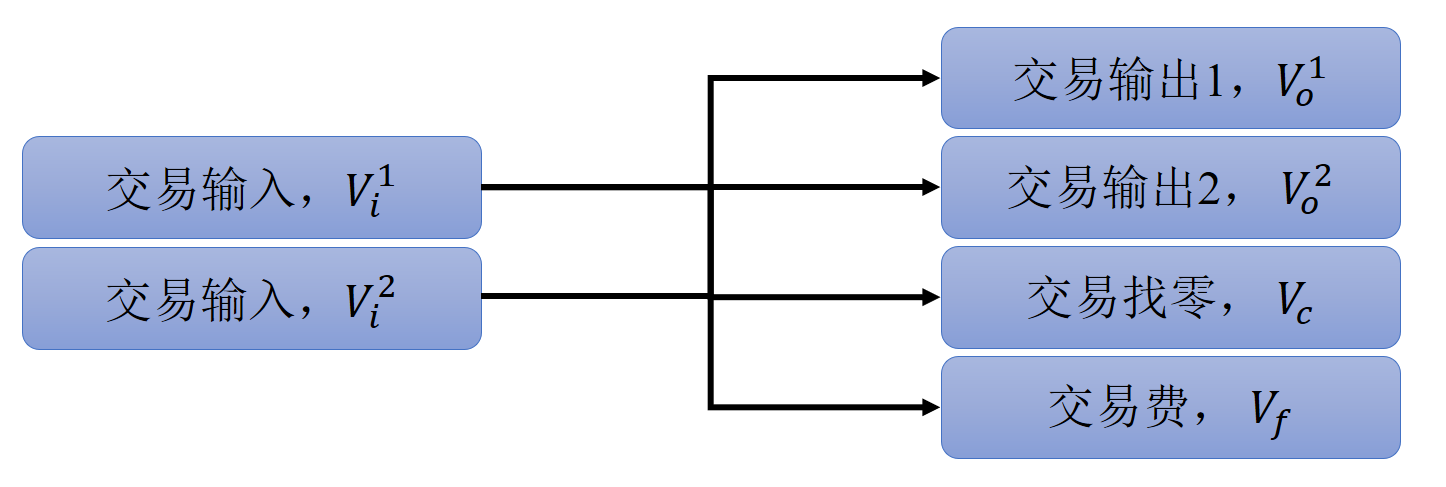
\includegraphics[width=0.75\textwidth]{figures/transaction.png}
    %\vspace{-0.1in}
    \caption{数字货币的交易流程}
    \label{fig:transaction}
\end{figure}

我们在这里给出数字货币交易的常见流程,如图\ref{fig:transaction}所示。
交易会包含至少一个交易输入$V_i$,同时对应若干个输出$V_o, V_c, V_f$。
其中$V_o$是正常交易输出;$V_c$是交易后剩余的找零,返回自己的账户;$V_f$是矿工交易费,
用于奖励矿工将这个交易打包至区块链中。在交易中,验证者需要确认交易的输入和交易的各项输出总和相等,
这样才能防止异常交易。当交易金额都是明文时,这个验证非常简单,
只需要普通加减法就可以验证。而当我们将实际交易金额都隐匿了以后,
想要验证这笔交易是否合法就困难了许多。

\section{零知识证明}

零知识证明最早由Goldwasser等人提出\cite{goldwasser1989knowledge}。
零知识证明是证明者向验证者证明某命题的方法,特点是证明过程中除``该命题为真''的事实以外,
证明者不会向验证者泄露任何资讯。普通的想向别人证明自己拥有该知识只需要对别人公开此知识内容即可,
但是这样会导致别人也知道了该知识,对自己造成损失。此时必须使用零知识证明才能在保护知识的同时,
让验证者相信证明者拥有该知识。

零知识证明可以如下形式化的定义:

\begin{itemize}
    \item 完备性:使用该证明方法,诚实的证明者确实可以向诚实的验证者证明自己持有知识。
    \item 健全性:使用该证明方法,不诚实的证明者,即未持有知识的证明者,
    能够向诚实的验证者证明自己持有该知识的概率可以忽略。
    \item 零知识:使用该证明方法证明完成后,验证者不能从中获取关于该知识的任何信息,
    也不能通过此次证明交互的内容假装成证明者,向别人证明自己或者证明者持有该知识。
    具体来说,将证明者和验证者交互的信息记录下来,由于完备性,
    任何人都能验证交互记录的合法;同时,任何不持有知识的人都能够伪造一份可以验证为合法的交互记录。
    这样说明了交互记录来自于所有可能的合法交互记录之一,和随机伪造的交互记录无法区分,
    因此没有从中透露任何信息。
\end{itemize}

\begin{figure}
    \centering
    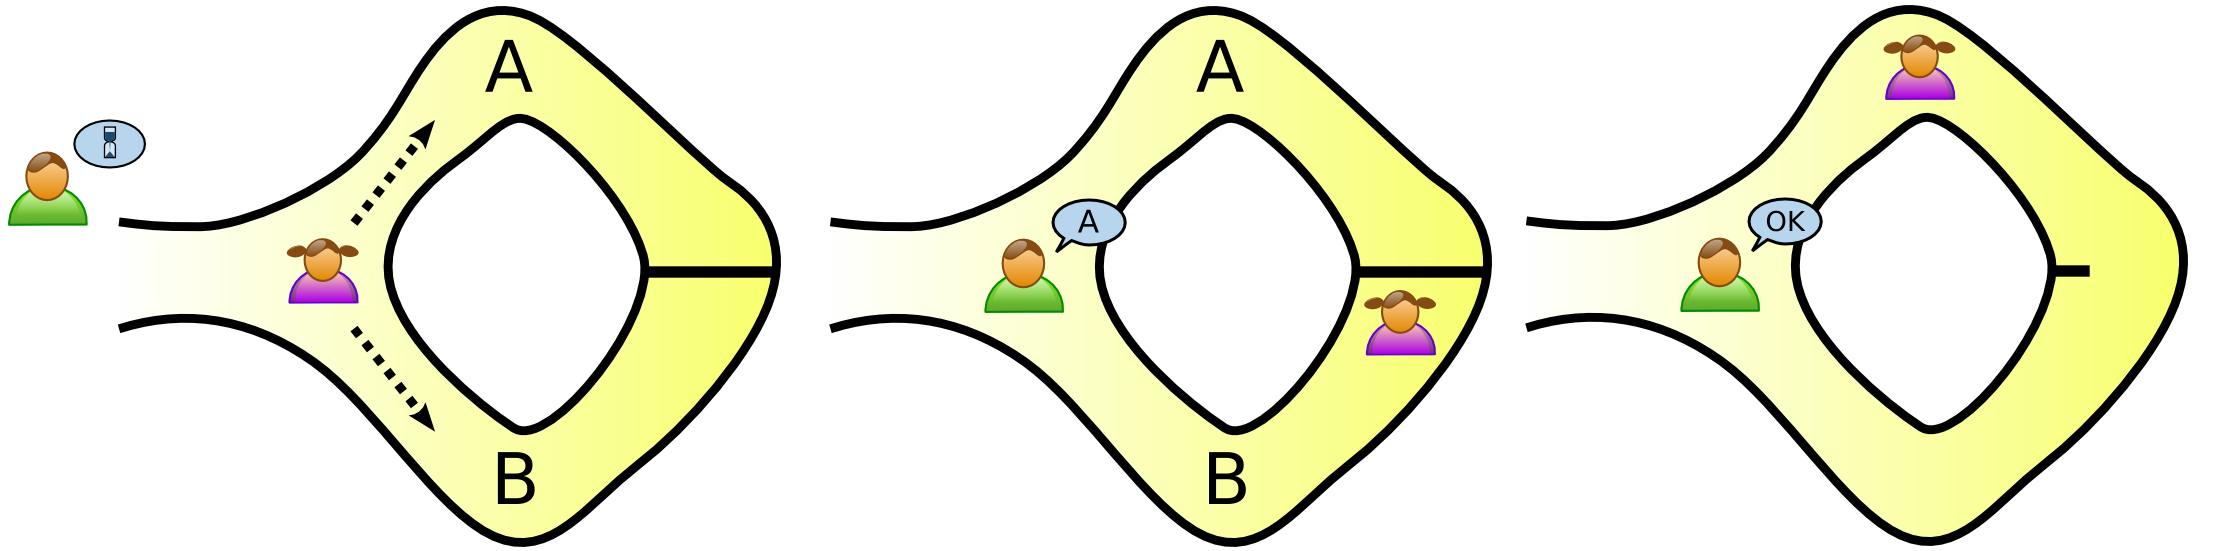
\includegraphics[width=\textwidth]{figures/alibaba.png}
    %\vspace{-0.1in}
    \caption{和零知识证明相关的寓言故事\cite{wikipedia_2021}}
    \label{fig:alibaba}
\end{figure}

对于零知识证明有一个形象的预言故事:在一座山中存在两条路,这两条路都没有岔路,
路的终点是同一扇门,如图\ref{fig:alibaba}所示。如果不打开这扇门就没法从一条路走到另一条路。
打开这扇门需要知道开门的密语,小红知道开门的密语,并且想向小绿证明这一点,
同时不想让小绿知道开门的密语。小绿需要先闭眼,让小红随机走一条路。
之后小绿告诉小红他选择的一条路,如果小红从他选择的路走回来了就算此次验证成功。
小绿和小红之间会进行很多次交互,如果小红每次都能从小绿指定的道路走回来,
那小绿就可以相信小红确实能够开门,同时小红也没有向小绿泄露开门的密语。

从零知识证明的定义分析,如果小红确实能开门,那么小红每次都能以100\%的概率从小绿指定的路回到路口,
这说明了该证明的完备性。而如果小红没有办法开门,那么每次小红都只有50\%的概率能够从指定路口回来,
只要交互次数达到了目标,小红能够通过证明的概率就可以忽略,说明了该证明的健全性。
最后,在这次证明中,小绿没有获得关于密语的任何信息,这从两方面说明。
首先小绿不能向任何人证明自己拥有该知识,由于小绿不知道密语,如果他向小黄证明,
由于小黄选择的随机道路和小绿可能不同,小绿无法利用和小红证明的过程帮助自己通过证明。
其次,小绿将该证明过程展示给其他人看时,例如将过程录制后再公开给小黄,
由于如果小红和小绿互相串通好了,实际上在证明开始前小红就知道了小绿的选择的话,
不论能不能打开门小红都能从小绿指定的道路走回来,
因此小黄不能通过这次证明过程就确定小红持有该密语。
该寓言故事中很重要的一点是小绿不能看到小红最开始是从哪条道路走的。如果小绿看到小红从道路A走,
那么他只要让小红从道路B走回来就说明小红持有密语,并且也无从得知密语;
但是这会导致该证明过程拿给任何人看都能让人推测出小红知道密语的事实,
因此也不算做零知识证明。

根据上述零知识证明的定义,结合交易金额隐匿的最终目标,
一个基于零知识证明的交易金额隐匿方法需要做到:

\begin{enumerate}
    \item 对于交易双方,可以查看交易的具体金额以及交易对象。
    这样才能够验证交易发起者确实完成了交易。
    \item 对于验证者,可以验证交易金额合法。这样保证了不会产生错误交易而导致凭空产生资金,
    同时却无法知道实际的交易金额。
\end{enumerate}

根据上述要求,在第\ref{chap:pedersen}章我们介绍数字总和承诺技术,
在第\ref{chap:bulletproof}章介绍数字范围证明技术。利用这两个技术,
验证者就能够验证交易输入和输出的数字总和相同,同时每个数字都在合法范围内。
同时交易双方通过约定承诺使用的遮罩数字,就可以查看实际的交易金额。